\section{Aim}
 To study the use of CURSOR in PLpg/SQL

\section{{Theory}}

PL/pgSQL cursor allows us to encapsulate a query and process each individual row at a time. We use cursors when we want to divide a large result set into parts and process each part individually. If we process it at once, we may have a memory overflow error.

In addition, we can develop a function that returns a reference to a cursor. This is an efficient way to return a large result set from a function. The caller of the function can process the result set based on the cursor reference.

\subsubsection{Syntax}

First we have to declare the cursor. There are two way to do that. 
\newline
1. Define a cursor variable. 
\begin{minted}{sql}
DECLARE my_cursor REFCURSOR;
\end{minted}
2. Bind a query to a cursor variable
\begin{minted}{sql}
cursor_name [ [NO] SCROLL ] CURSOR [( name datatype, name data type, ...)] FOR query;
\end{minted}
Next, we open the cursor.\newline
To open an unbound cursor:
\begin{minted}{sql}
OPEN unbound_cursor_variable [ [ NO ] SCROLL ] FOR query;
\end{minted}
\newline
To open an bound cursor:
\begin{minted}{sql}
OPEN cursor_variable
\end{minted}
Now we can fetch each row from the query output into a variable. 
\begin{minted}{sql}
FETCH [ direction { FROM | IN } ] cursor_variable INTO target_variable;
\end{minted}
where target\_variable is a variable of type record, row, or a comma seperated list of variables.

\section{{Code and Output}}

\begin{enumerate}
\item Create table student (id, name, m1, m2, m3, grade). Insert 5 tuples into it. Find the total, calculate grade and update the grade in the table.
\begin{minted}{sql}

CREATE OR REPLACE FUNCTION grader()
RETURNS INTEGER
AS $$
DECLARE
cur CURSOR FOR SELECT * FROM student;
rec RECORD;
total INTEGER;
grd CHAR(1);
BEGIN
OPEN cur;
LOOP
total := 0;
FETCH cur into rec;
EXIT WHEN NOT FOUND;
total := rec.m1 + rec.m2 + rec.m3;
IF total > 250 THEN
grd := 'A';
ELSIF total > 200 THEN
grd := 'B';
ELSIF total > 150 THEN
grd := 'C';
ELSIF total > 100 THEN
grd := 'D';
ELSE
grd := 'F';
END IF;
UPDATE student SET grade = grd WHERE CURRENT OF cur;
END LOOP;
CLOSE cur;
RETURN null;
END;
$$ LANGUAGE plpgsql;
\end{minted}

\newline
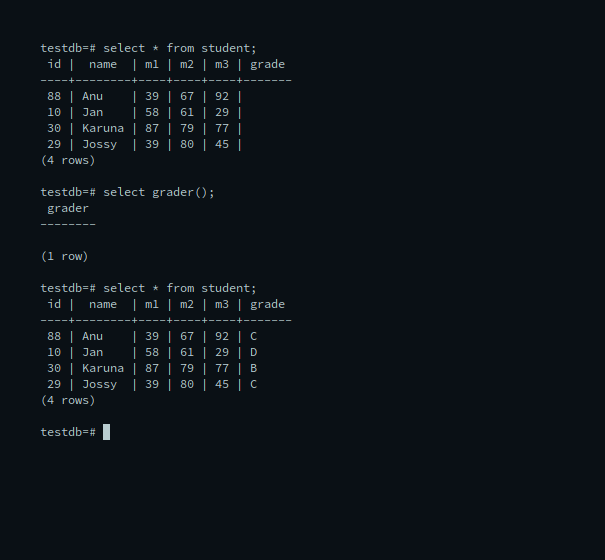
\includegraphics[width=\linewidth]{../Images/Cursors/1.png}

\item Create bank\_details (accno, name, balance, adate).Calculate the interest of the amount and insert into a new table with fields (accno, interest). Interest = 0.08 * balance.\newline

\newline
\begin{minted}{sql}

CREATE OR REPLACE FUNCTION interest()
RETURNS INTEGER
AS $$
DECLARE
cur CURSOR FOR SELECT * FROM bank_details;
rec RECORD;
intr REAL;
BEGIN
CREATE TABLE bank_new(acc_no int, interest real);
OPEN cur;
LOOP
FETCH cur into rec;
EXIT WHEN NOT FOUND;
intr := rec.balance * 0.08;
INSERT INTO bank_new VALUES(rec.accno, intr);
END LOOP;
CLOSE cur;
RETURN null;
END;
$$ LANGUAGE plpgsql;
\end{minted}

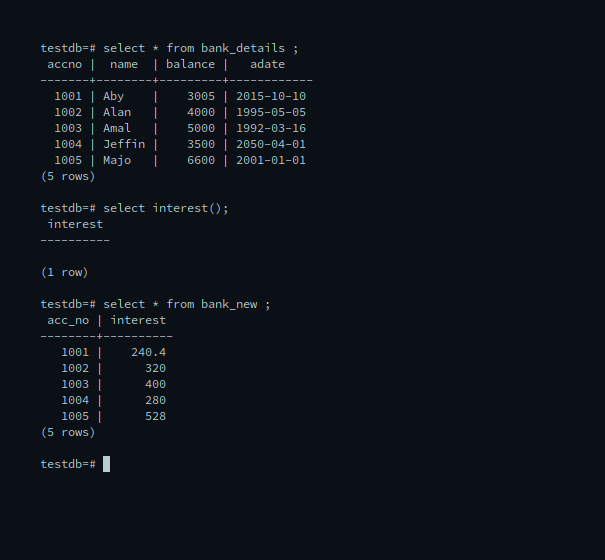
\includegraphics[width=\linewidth]{../Images/Cursors/2.png}

\item Create table people\_list (id, name, dt\_joining, place).If person’s experience is above 10 years, put the tuple in table exp\_list (id, name, experience).\newline
\begin{minted}{sql}

CREATE OR REPLACE FUNCTION exp()
RETURNS INTEGER
AS $$
DECLARE
cur CURSOR FOR SELECT * FROM people_list;
rec RECORD;
BEGIN
OPEN cur;
LOOP
FETCH cur into rec;
EXIT WHEN NOT FOUND;
IF rec.dt_joining < '2009-08-18' THEN
INSERT INTO exp_list VALUES
	(rec.id, rec.name, ('2019-08-18' - rec.dt_joining)/365);
END IF;
END LOOP;
CLOSE cur;
RETURN null;
END;
$$ LANGUAGE plpgsql;
\end{minted}

\newline
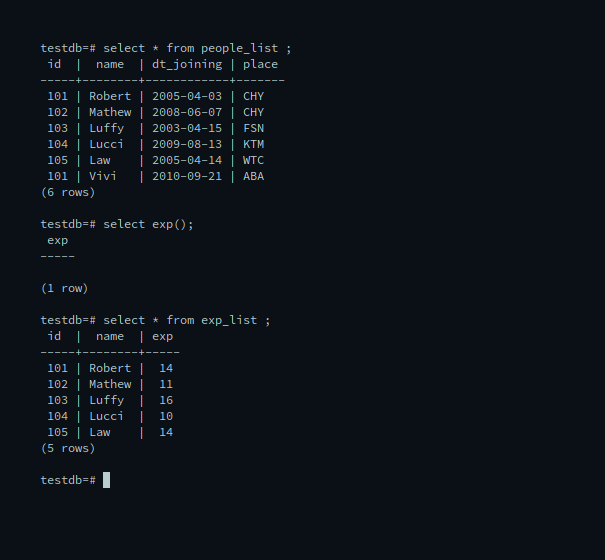
\includegraphics[width=\linewidth]{../Images/Cursors/3.png}
\item Create table
employee\_list(id,name,monthly salary). If:\newline
annual salary less than 60000, increment monthly salary by 25\% \newline
between 60000 and 200000, increment by 20\%\newline
between 200000 and 500000, increment by 15\%\newline
annual salary greater than 500000, increment monthly salary by 10\%\newline
\begin{minted}{sql}

CREATE OR REPLACE FUNCTION sal()
RETURNS INTEGER
AS $$
DECLARE
cur CURSOR FOR SELECT * FROM employee_list;
rec RECORD;
BEGIN
OPEN cur;
LOOP
FETCH cur into rec;
EXIT WHEN NOT FOUND;
IF (rec.salary * 12) < 60000 THEN
UPDATE employee_list 
	SET salary = salary * 1.25 
	WHERE CURRENT OF cur;
ELSIF (rec.salary * 12) < 200000 THEN
UPDATE employee_list 
	SET salary = salary * 1.2 
	WHERE CURRENT OF cur;
ELSIF (rec.salary * 12) < 500000 THEN
UPDATE employee_list 
	SET salary = salary * 1.15 
	WHERE CURRENT OF cur;
ELSE
UPDATE employee_list 
	SET salary = salary * 1.1 
	WHERE CURRENT OF cur;
END IF;
END LOOP;
CLOSE cur;
RETURN null;
END;
$$ LANGUAGE plpgsql;
\end{minted}

\newline
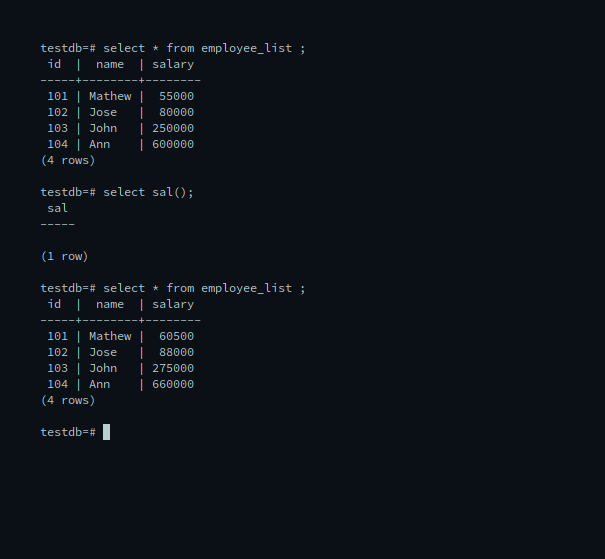
\includegraphics[width=\linewidth]{../Images/Cursors/4.png}

\end{enumerate}

\section{Result}
Implemented the program for Cursors using Postgresql 11.5 on Manjaro Linux and the output was obtained.